\documentclass{beamer}
\usetheme{uic}
\usepackage{amsfonts,amsmath,oldgerm,algorithmic,algorithm}
\usepackage[font=small,labelfont=bf]{caption} % Required for specifying captions to tables and figures
\usepackage{graphicx} % Required for inserting images

\usepackage{listings}
\usepackage{xcolor} % For custom colors (optional)
\usepackage{caption}
\usepackage{svg}
\usepackage{pgfgantt}
\usepackage{caption} % Add this to your preamble if not already included


\captionsetup[figure]{labelformat=empty} % Removes the label (e.g., "Figure")


\newcommand{\hrefcol}[2]{\textcolor{uihteal}{\href{#1}{#2}}}
\newcommand{\testcolor}[1]{\colorbox{#1}{\textcolor{#1}{test}}~\texttt{#1}}

% Please see Section 18.1 of Beamer User Guide for all the options \usefonttheme provides
\usefonttheme[onlymath]{serif}
% \usefonttheme{serif} % use this if you would like Serif font throughout (and not just for math)

\title{Functionally-Complete Boolean Logic in Real DRAM Chips:
Experimental Characterization and Analysis}


\titlebackground*{images/uic_lockup_2.png}

% NOTE 1: The asterisk splits the background image. This option is good
% for logo-based backgrounds. If you use an image based background
% it's recommended to not split it:

% \titlebackground{images/uic_seo.jpg}

% NOTE 2: If you use a title background that does not have a logo, you might
% want to enable logo in the top left.
% To do that, simply comment out this line
\themecolor{lightnologo}

\subtitle{%
Paper Review by: \\%
Ali Asghar(21PWCSE2059) \\[1em]%
CSE-420 Embedded Systems \\
Course Instructor: Dr. Asif Ali Khan \\%
%Advisor: Dr. Laiq Hassan \\[1em]
%FYP Progress-I Presentation%
}

% This can be adjusted accordingly for longer titles
\newcommand{\titleboxwidth}{0.65\textwidth}

%\author{\href{mailto:umunee2@uic.edu}{Usama Muneeb}}
\date{}

\begin{document}
\maketitle
\themecolor{light} % reverts to a logo based theme (if you disabled it for title page)

% default is no footline, but page numbers are incredibly useful for the audience to ask questions later
\footlinecolor{uicblue}


%\begin{frame}[t]{Overview}
%	\begin{itemize}
%			\item Introduction
%			\item Key Contributions
%			\item Experimental Methodology
%			\item Findings and Results
%			\item Implications and Future Work
%	\end{itemize}
%\end{frame}

\begin{frame}[t]{Introduction}
	\begin{itemize}
			\item \textbf{Problem:} Data movement
			\item \textbf{Solution:} Processing-using-DRAM (PuD) 
			\item \textbf{Previous Work:} Basic bitwise operations (AND, OR) but lacked functionally complete logic.
	\end{itemize}
\end{frame}

%\begin{frame}[t]{Key Contributions}
%\begin{enumerate}
%    \item Functionally complete Boolean operations (NOT, NAND, NOR) in off-the-shelf DRAM.
%    \item Many-input (up to 16-input) AND, OR, NAND, and NOR.
%    \item Reliability across 256 DDR4 DRAM chips (success rate).
%    \item Open-source infrastructure.
%\end{enumerate}
%\end{frame}

%\begin{frame}[t]{Experimental Methodology}
%\framesubtitle{Setup and Testing}
%\begin{itemize}
%    \item \textbf{Hardware:} FPGA-based testing infrastructure (DRAM Bender).
%    \item \textbf{Tests:} Conducted on 256 DDR4 DRAM chips from SK Hynix and Samsung.
%    \item \textbf{Parameters:} Evaluated success rates under varying data patterns, temperatures (50°C–95°C), and DRAM configurations.
%\end{itemize}
%\end{frame}

\begin{frame}[t]{NOT Gate Implementation}
\framesubtitle{}
\begin{figure}
	\centering
		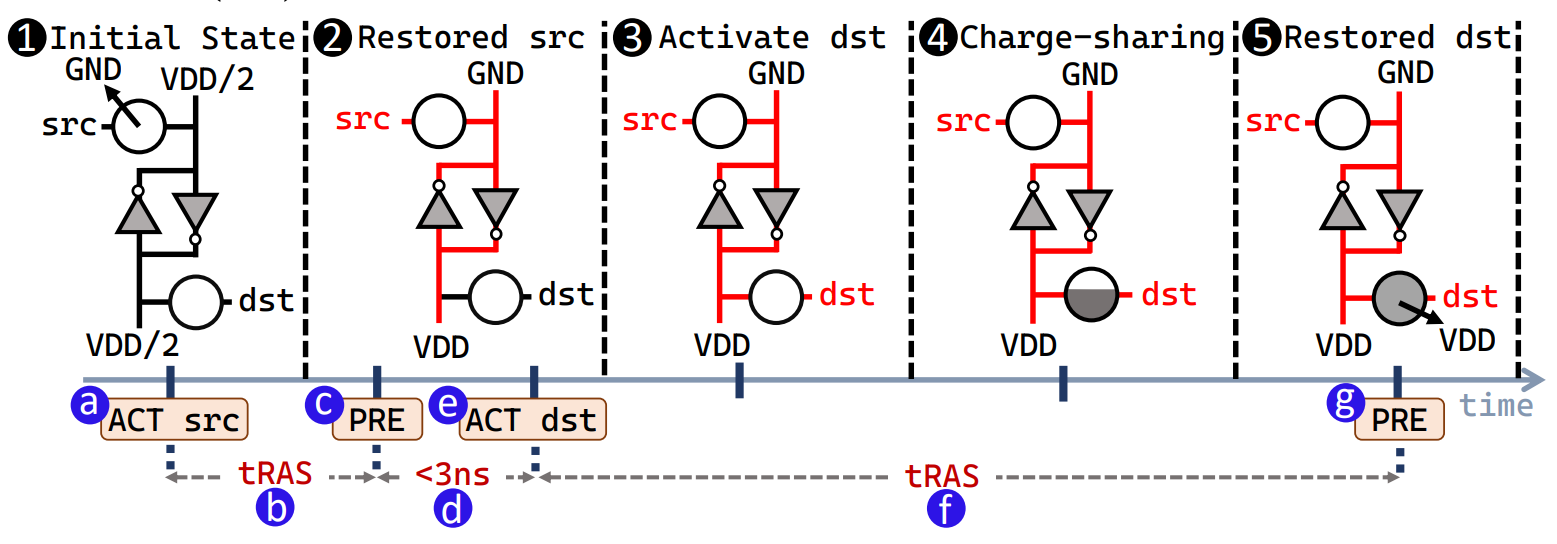
\includegraphics[width=0.95\textwidth]{images/NOT.png}
	\caption{}
	\label{fig:NOT}
\end{figure}
\end{frame}

\begin{frame}[t]{AND and NAND Gate Implementation}
\framesubtitle{}

\begin{figure}
	\centering
		\includegraphics[width=0.85\textwidth]{images/AND\_NAND.png}
	\caption{}
	\label{fig:NOT}
\end{figure}

\end{frame}

%\begin{frame}[t]{DRAM Subarray Boundery}
%\framesubtitle{}
%\begin{itemize}
%	\item Boundary is found by Reverse Engineering
%	\item Using the RowClone method
%	\item if after RowClone, src = dst then same subarray.
%	\item else different subarray.
%\end{itemize}
%\end{frame}

%\begin{frame}{Findings}
%\framesubtitle{Reliability of Boolean Operations}

%\begin{table}[h]
%    \centering
%		\setlength{\arrayrulewidth}{0.5mm} % Adjust the thickness of the table lines
%    \captionsetup{skip=0pt} % Adjust the spacing between caption and table (default is 10pt)
%    \caption{Reliability of Boolean Operations}
%		\vspace{-10pt} % Add negative vertical space if additional reduction is needed
%    \resizebox{\textwidth}{!}{ % Resize table to fit the frame width
%        \begin{tabular}{|p{1cm}|p{3cm}|p{3cm}|} 
%            \hline
%            \textbf{No.} & \textbf{Operation} & \textbf{Reliability} \\ \hline
%            1 & NOT  & 98.37\% \\ \hline
%            2 & 16-input NAND & 94.94\% \\ \hline
%            3 & 16-input NOR & 95.87\%  \\ \hline
%            4 & 16-input AND & 94.94\% \\ \hline
%            5 & 16-input OR &  95.85\% \\ \hline
%        \end{tabular}
%    }
%\end{table}
%\end{frame}

%\begin{frame}{Experimental Results}
%\framesubtitle{Key Observations}
%\begin{itemize}
%    \item \textbf{NOT Operation:} Reliable across all tested DRAM chips with a high success rate.
%    \item \textbf{Many-Input Logic: }Up to 16-input NAND/NOR/AND/OR possible with robust performance.
%    \item \textbf{Resilience:} DRAM chips showed minimal impact from temperature fluctuations or input pattern variations.
%\end{itemize}
%\end{frame}

%\begin{frame}{Implications and Future Work}
%\begin{itemize}
%    \item \textbf{Potential:} DRAM as a computational substrate to reduce data movement bottlenecks.
%    \item \textbf{Challenges:} Variability in performance across manufacturers and DRAM types.
%    \item \textbf{Future Directions:}
%    \begin{itemize}
%        \item Optimizing DRAM designs for in-memory computing.
%        \item Leveraging open-source infrastructure for broader research.
%    \end{itemize}
%\end{itemize}
%\end{frame}

\backmatter
\end{document}